%%%%%%%%%%%%%%%%%%%% author.tex %%%%%%%%%%%%%%%%%%%%%%%%%%%%%%%%%%%
%
% sample root file for your "contribution" to a contributed volume
%
% Use this file as a template for your own input.
%
%%%%%%%%%%%%%%%% Springer %%%%%%%%%%%%%%%%%%%%%%%%%%%%%%%%%%


% RECOMMENDED %%%%%%%%%%%%%%%%%%%%%%%%%%%%%%%%%%%%%%%%%%%%%%%%%%%
\documentclass[graybox]{svmult}

% choose options for [] as required from the list
% in the Reference Guide

\usepackage{type1cm}        % activate if the above 3 fonts are
                            % not available on your system
%
\usepackage{makeidx}         % allows index generation
\usepackage{graphicx}        % standard LaTeX graphics tool
                             % when including figure files
\usepackage{multicol}        % used for the two-column index
\usepackage[bottom]{footmisc}% places footnotes at page bottom


\usepackage{newtxtext}       % 
\usepackage{newtxmath}       % selects Times Roman as basic font

% see the list of further useful packages
% in the Reference Guide

\makeindex             % used for the subject index
                       % please use the style svind.ist with
                       % your makeindex program

%%%%%%%%%%%%%%%%%%%%%%%%%%%%%%%%%%%%%%%%%%%%%%%%%%%%%%%%%%%%%%%%%%%%%%%%%%%%%%%%%%%%%%%%%

\begin{document}

\title*{Multi-Agent Reinforcement Learning for the Energy Optimization of Cyber-Physical Production Systems}
\titlerunning{MARL for the Energy Optimization of CPPS}
% Use \titlerunning{Short Title} for an abbreviated version of
% your contribution title if the original one is too long
\author{Jupiter Bakakeu*, Shirin Baer, Hans-henning Klos, Joern Peschke, Matthias Brossog and Joerg Franke}
% Use \authorrunning{Short Title} for an abbreviated version of
% your contribution title if the original one is too long
\authorrunning{Jupiter Bakakeu et al.}
\institute{Jupiter Bakakeu, Matthias Brossog and Joerg Franke \at Friedrich-Alexander-Universität Erlangen-Nürnberg, Egerlandstr. 7-9, 91058 Erlangen, Germany, \email{jupiter.bakakeu@faps.fau.de, matthias.brossog@faps.fau.de, joerg.franke@faps.fau.de}
\and Shirin Baer, Hans-henning Klos and Joern Peschke\at Siemens AG, Gleiwitzer Str. 555, 90475 Nuremberg, Germany, \email{schirin.baer@siemens.com, hans-henning.klos@siemens.com, joern.peschke@siemens.com}}
%
% Use the package "url.sty" to avoid
% problems with special characters
% used in your e-mail or web address
%
\maketitle

\abstract*{This chapter proposes an artificial intelligence based solution for the efficient operation of a heterogeneous cluster of flexible manufacturing machines with energy generation and storage capabilities in an electricity micro-grid featuring a high volatility of electricity prices. The problem of finding the optimal control policy is first formulated as game theoretic sequential decision making problem under uncertainty, where at every time step the uncertainty is characterized by future weather dependent energy prices, high demand fluctuation, as well as random unexpected disturbances on the factory floor. Because of the parallel interaction of the machines with the grid, the local viewpoints of an agent are non-stationary and non-Markovian. Therefore, traditional methods such as standard reinforcement learning approaches that learn a specialized policy for a single machine are not applicable. To address this problem, we propose a multi-agent actor-critic method that takes into account the policies of other participants to achieve explicit coordination between a large numbers of actors. We show the strength of our approach in mixed cooperative and competitive scenarios where different production machines were able to discover different coordination strategies in other to increase the energy efficiency of the whole factory floor.}

\abstract{This chapter proposes an artificial intelligence based solution for the efficient operation of a heterogeneous cluster of flexible manufacturing machines with energy generation and storage capabilities in an electricity micro-grid featuring a high volatility of electricity prices. The problem of finding the optimal control policy is first formulated as game theoretic sequential decision making problem under uncertainty, where at every time step the uncertainty is characterized by future weather dependent energy prices, high demand fluctuation, as well as random unexpected disturbances on the factory floor. Because of the parallel interaction of the machines with the grid, the local viewpoints of an agent are non-stationary and non-Markovian. Therefore, traditional methods such as standard reinforcement learning approaches that learn a specialized policy for a single machine are not applicable. To address this problem, we propose a multi-agent actor-critic method that takes into account the policies of other participants to achieve explicit coordination between a large numbers of actors. We show the strength of our approach in mixed cooperative and competitive scenarios where different production machines were able to discover different coordination strategies in other to increase the energy efficiency of the whole factory floor.}

\section{Introduction}
\label{sec:1}

Today the cost-efficient and stable supply of energy for production processes is a topic of increasing relevance. Changes in the structure of power generation towards decentralized systems and the growing share of renewable energy sources such as photovoltaics and wind power lead to a volatile situation in the supply of electrical energy. The concept in which electricity generation solely follows a demand based on statistical forecasts is no longer applicable. As a consequence, new concepts that harness the flexibility of energy consumption on the consumer side are becoming increasingly important, resulting in new developments in energy markets where a flexible consumer can get incentives for providing flexibility and participating in specific programs.

In this context, cyber-physical production systems (CPPS) with multiple possible plant topologies and the ability to produce huge number of product variants can make a significant contribution to a transition to a flexible energy demand. However, ensuring such flexibility in the industry 4.0 context requires a sophisticated control strategy to intelligently supervise the power consumption of the underlying components at every given time so that the total energy consumption follows given load profile boundaries. Moreover, the control strategy has to ensure a high productivity while coping with the uncertainties that can arise from the high fluctuations of weather-dependent energy prices, fast market changes as well as random unexpected disturbances in the factory floor.

Traditionally, analytical and simulation-based approaches are used to compute the optimal control strategy for the connected loads, distributed generation and storage components. However, these approaches often require complex models with precise descriptions of system features and functions. The engineering efforts for these systems are often a crucial aspect, which restricts implementations in the large scale. This problem becomes even more important in the industry 4.0 context, where fast market changes can lead to frequent changes in product and process configurations and therefore to the system models.

For these reasons, model-free control solutions and especially new artificial intelligence algorithms are considered as valuable alternatives or supplements \cite{Gholian7236921}. One of the most popular model-free control paradigms that has gained in importance in recent years is Reinforcement Learning (RL) \cite{Sutton9780262039246, bakakeu2018}: a model-free algorithm that does not require system identification steps or apriori knowledge. While being very popular in single agent settings (see \cite{mnih2013playing}, \cite{openai2019solving}, \cite{hausknecht2015deep}, \cite{schulman2017proximal}), a naive application of RL in a multi-agent environment  (as it is the case for CPPS) is likely to perform poorly. One issue is the non-Markovian nature of the resulting environment: since the action of one agent can affect the outcome of the action of other agents, the single perspective of an agent, which mainly consists of partial observations, becomes non-stationary in the sense that changes that cannot only be explained by the inherent stationary dynamics of the environment can occur. It is therefore important to coordinate the choices of actions of all agents in order to achieve the intended effects. Furthermore, an agent trained in a single environment setting is inherently bounded by the task description. A slight modification of the task or an evolution of the environment creates new pressures for retraining.

In order to solve these problems, many have worked on unsupervised exploration and skill acquisition methods such as \textit{intrinsic motivation} and \textit{self-play}. Rather than training the agents to solve a specific task in a predefined environment, the agent are conditioned in a autocurricula environment whereby the agents have to continuously coordinate their strategies (via competition or cooperation) in order to solve an ever evolving task. As a result, the agents learn an ensemble of emergent skills and coordination strategies rather than a specific complex policy making them more robust to environment changes.

There has been much success in leveraging multi-agent autocurricula to solve multi-agent problems such as \cite{lowe2017multiagent} and \cite{bansal2017emergent} both in discrete and continuous real-time domains. In both cases, self-play approaches provided the agents with a perfectly tuned curriculum. The success in these settings inspires confidence that inducing autocurricula in physically grounded and open-ended environments such industrial micro-grids could eventually enable the agents controlling the grid components to acquire an unbounded number of robust and emergent skills that can lead to a global resource optimization. In this chapter, we investigate whether the idea of autocurricula multi-agent reinforcement learning environments can yield fruit in solving the problem of the energy optimization of an heterogeneous cluster of cyber-physical production systems with energy generation and storage capabilities in an electricity micro-grid featuring a high volatility of electricity prices.

In more detail, we first formulate the energy optimization problem as an observable Markov game which we then use to design an autocurricula environment that simulates a micro-grid of flexible manufacturing machines with energy generation and energy storage capabilities. We then introduce several multi-agent tasks with comparative goals, where the different agents would need to learn not only highly developed skills but also coordinate the learned strategies in order to achieve the intended global effect. We then train the agents using a distributed implementation of a recent policy gradient algorithm, Proximal Policy Optimization (PPO) \cite{schulman2017proximal} in a framework of centralized training with decentralized execution. By adding a simple exploration curriculum to aid exploration in the environment, we found that in both cooperative and competitive scenarios different production machines were able to discover different coordination strategies in other to increase the energy efficiency of the whole factory floor.

The remainder of this chapter is structured as follows. In section \ref{sec:2}, backgrounds and related work on load management systems as well as multi-agent reinforcement learning algorithms are presented. Then, we formulate the energy optimization problem as a sequential decision making problem under uncertainty in section \ref{sec:3}. Section \ref{sec:4} gives a detailed description of our training algorithm and the autocurricula environment. Experimental results demonstrating the strength of our approach are presented in section \ref{sec:5}. Finally, we summarize the paper and discuss some directions for future work in section \ref{sec:6}.


\section{Backgrounds and Related Work}
\label{sec:2}
\subsection{Load Management Systems}

A growing number of works on load management systems have primarily focused on industrial load control and have generally ignored the volatility of the energy prices \cite{Gholian7236921, CHEN2015263, Wang6345296, MIDDELBERG20091266}. Most recent works \cite{Sun6329376, DUFLOU2012587, Pechmann2011} took into account this factor and showed that analytical approaches can be used to compute the optimal time to change the energetic state of a machine for energy control purposes without sacrificing the system throughput. Energy-aware scheduling was also considered to optimize the production plan using mixed integer programming \cite{BRUZZONE2012459, FANG2011234}. However, all the proposed solutions rely on fixed product and machine configurations and thus not applicable in a dynamic context. Furthermore, these solutions require a precise estimation of the model of the production machine as well as the associated parameters. Since the acquisition of such models mostly rely on expert knowledge, the proposed solutions are not scalable and not cost effective. In this chapter, we focus on a model-free control solution that use RL and do not require an explicit system identification.

\subsection{Reinforcement Learning}
Reinforcement learning (RL) is one of the main classes of machine learning methods that has been successfully applied to solve sequential decision-making problem under uncertainties \cite{Liu6918520}. In such a setting, an agent learns to act using a (partial observable) Markov decision process (MDP) \cite{Sutton9780262039246} formalism. At each time step, the agent selects an action from a finite set of possible actions. After executing the selected action, the environment is updated and the agent receives a rewards signal, which can also be interpreted as a punishment from the environment. The goal of the agent is to maximize the discounted reward in the long run. To achieve this, the agent has to compute the optimal policy based on interactive learning with the environment (see Fig. 1).

% For figures use
%
\begin{figure}[b]
\sidecaption
% Use the relevant command for your figure-insertion program
% to insert the figure file.
% For example, with the graphicx style use
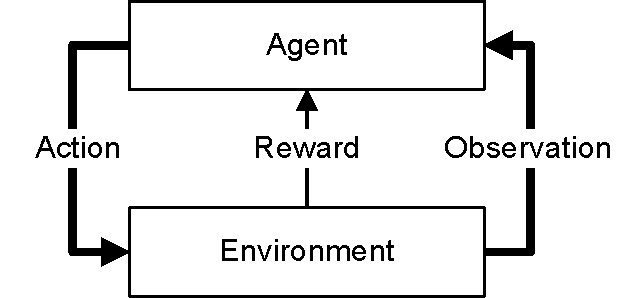
\includegraphics[scale=.65]{images/Single_Agent_RL.pdf}
%
% If no graphics program available, insert a blank space i.e. use
%\picplace{5cm}{2cm} % Give the correct figure height and width in cm
%
\caption{The agent-environment interaction in Reinforcement Learning.}
\label{fig:1}       % Give a unique label
\end{figure}


The literature provide many examples of RL algorithms applied to energy management problems. In 1996. Anderson et al. applied Q-learning to modulate the output of the PI controller for a heating coil \cite{ANDERSON1997421, Li6519950}. In the same direction, Ruelens et al.\cite{Ruelens7038106, Ruelens7792709}, De Somer et al. \cite{Somer8260152} and Kazmi et al. \cite{KAZMI2018159} were able to apply RL methods to reduce the domestic water heating costs. Jiang et al. implemented a hierarchical multi-agent Q learning approach for dynamic demand response and distributed energy resource management in a micro-grid \cite{Jiang6912013}. In recent studies \cite{ANVARIMOGHADDAM201741, prasad2018multiagent, LU2018220}, the authors implemented a multi-agent DQN approach where each agent controlled a house. The agent could consume/store energy, request energy from or grant energy to neighbors, deny energy to neighbors or purchase it from the grid.

\subsection{Multi-Agent Reinforcement Learning}
In multi-agent reinforcement learning (MARL), multiple agents perform concurrently in a single environment \cite{Littman1994multiagent, Hu1998MultiagentRL, Busoniu4445757, Tan93multiagentreinforcement}.  The simplest approach to learning in multi-agent settings is to train each agent independently. This was attempted with Q-learning in \cite{Tan93multiagentreinforcement}, but does not perform well in practice \cite{Matignon2012IndependentRL} since many applications assume interdependency between the agents. More recently, deep neural networks have been successfully used in RL to approximately represent policy and value functions. It is therefore not surprising that deep neural networks have also been applied to MARL settings \cite{tampuu2015multiagent, Gupta71682}, allowing multi-agent learning in high-dimensional/continuous state spaces. However, applying standard RL methods to MARL problems is  challenged by some limitations, such as non-stationary of the environment from the perspective of individual agents \cite{foerster2017stabilising, Lowe2017MultiAgentAF, Foerster2017CounterfactualMP}, lack of coordination/communication in cooperative settings \cite{Lowe2017MultiAgentAF, NIPS2016_6398, MordatchA17, FoersterAFW16a}, credit assignment in cooperative settings with global rewards \cite{Foerster2017CounterfactualMP, Rashid2018,Sunehag3238080}, and the failure to take opponent strategies into account when learning agent policies \cite{He3045581}.

Most relevant to this work are recent approaches \cite{MordatchA17, Foerster2017CounterfactualMP} that propose an actor-critic framework consisting of centralized training with decentralized execution as well as some approaches that utilize attention in a fully centralized multi-agent setting \cite{Choi2017MultifocusAN, Jiang3327828}. The proposed method uses separate centralized critics for each agent, which take all other agent’s actions and observations as input during the training phase, and  actors whose policies are conditioned only on local information. This practice reduces the non-stationary of multi-agent environments, as considering the actions of other agents to be part of the environment makes the state transition dynamics stable from the perspective of one agent. In practice, these ideas greatly stabilize learning because of the reduced variance in the value function estimates.

Our proposed solution follows these recent developments and propose a centralized critic for PPO applied in a multi-agent setting. It is more flexible than the aforementioned approaches in the sense that it is able train policies in environments with any reward setup, observation and action spaces making it broadly applicable to different environment types including industrial micro-grid environments.




\section{System Model and Problem Formulation}
\label{sec:3}
The chapter addresses the problem of optimally controlling an industrial micro-grid featuring a large share of renewable energy and a high volatility of electricity prices. We consider a micro-grid as a localized group of energy sources, loads and storage components that can operate in two distinct modes: grid-connected mode and isolated mode. In grid-connected mode, the micro-grid system has the possibility to buy/sell energy from/to the macro-grid in order to meet the load demand. The challenge in connected mode is to reduce the total energy cost. In isolated mode, the micro-grid can function autonomously in the sense that enough energy can be generated in the grid to supply the loads. In this case the challenge is to meet the load demand and to balance the power flow between the components of the grid. In our setting, the grid is executed in mixed mode. In other words, the industrial micro-grid, we are considering, can switch from one mode to another.

\subsection{System Model}
\label{subsec:31}

% For figures use
%
\begin{figure}[b]
%\sidecaption
% Use the relevant command for your figure-insertion program
% to insert the figure file.
% For example, with the graphicx style use
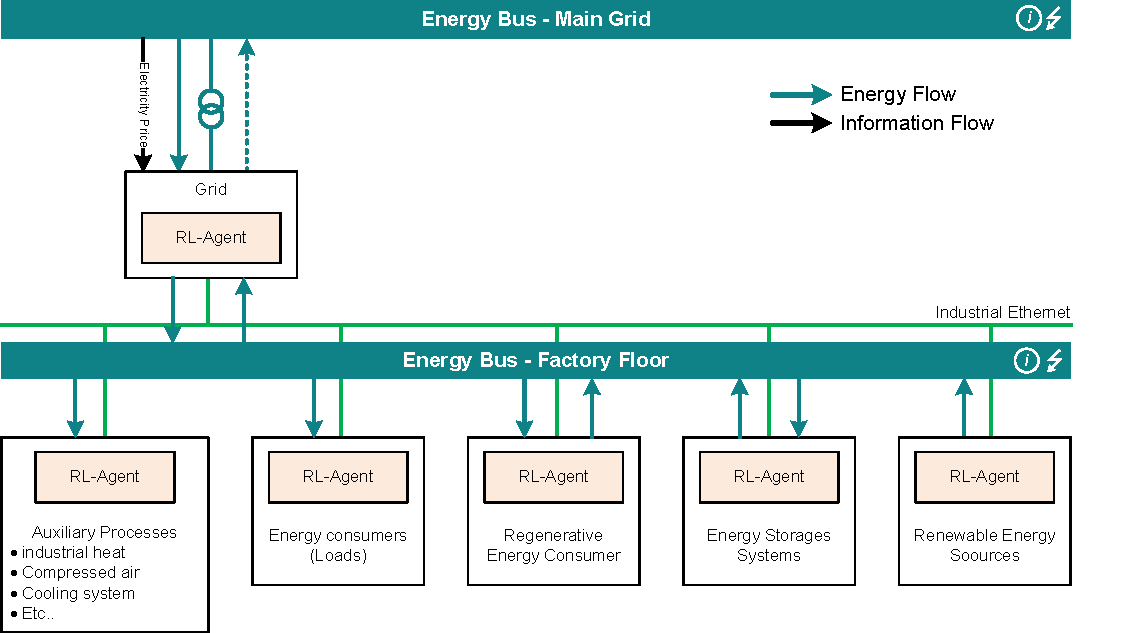
\includegraphics[scale=.65]{images/System_Model}
%
% If no graphics program available, insert a blank space i.e. use
%\picplace{5cm}{2cm} % Give the correct figure height and width in cm
%
\caption{System Overview. Every grid-component is controlled by a reinforcement learning agent.}
\label{fig:system_model}       % Give a unique label
\end{figure}

As illustrated in Fig.\ref{fig:system_model}, the micro-grid system consists of the following components: renewable energy sources such as PV-Arrays, electricity loads representing production machines, regenerative energy consumers, energy storages systems such as batteries and auxiliary process loads for air compressors and cooling systems. The components share the same energy bus, enabling a transfer of electrical energy between the components. The proposed system model is equally applicable to ac and dc micro-grids and a simple formal description of the components can be described as follow:
\begin{itemize}
\item{\textit{\textbf{ Renewable energy sources}} are renewable energy generators such as PV-Arrays or wind turbines. The power generated depends on environmental and weather factors such as solar radiation profile and wind speed. It is therefore not predictable. Energy generators are characterized by two operating states: $on$ and $off$. The generators are considered to be in the $off$-state when the electrical power generated by the energy sources is negligible for example because of weather conditions such as cloudy weather or nighttime. We assume that if the generators are not in $off$ state, then the power generated is constant and equal to the maximum electricity power that can be produced by the source. Therefore
%
\begin{equation}
 P_G = 
 \begin{cases}
      0 & \text{if}\ state=off \\
      P_Gmax & \text{otherwise}
    \end{cases} \;
\end{equation}
%
 } 
\item{\textit{\textbf{Energy storage systems}}. In order to take full advantage of renewable energy sources, it is vital to have energy storage systems capable of handling variations in energy production. In our environment, we consider batteries or super-capacitor systems that consume a constant energy when charging and produce a constant energy when discharging. In addition, the operation of energy storage systems has to be carefully designed and controlled to protect them from damages that are: overcharging and overdischarging. Therefore, each storage system is also characterized by a maximum and minimum state-of-charge (SoC). The energy storage systems have three required states: $charging$, $discharging$ and $idle$. The electrical power consumed or released by the component highly depends on the current operational state and the component\rq{s} state-of-charges.}
 
 \item{\textit{\textbf{Energy loads}} represent production machines that consume energy in order to execute a production task. A production machine can have different operation states: $powered off$, $executing$, $stand by$, etc… Depending on the production task and the operation state, a production machine can follow a predefined or a characteristic load profile. For a fixed set of production tasks, the load profile of a machine can be measured and approximated. In our setting, we consider 3 basic load profile as illustrated in Fig. \ref{fig:load_profile}. Any machine\rq{s} load profile can be seen as a linear combination of this basic load profiles. In isolated mode, the micro-grid cannot guarantee continuous power supply to the load because it is often influenced by the unpredictable power generation. When the generated power is not able to drive the loads, the noncritical loads must shut down.}
 
 % For figures use
%
\begin{figure}[h!]
%\sidecaption
% Use the relevant command for your figure-insertion program
% to insert the figure file.
% For example, with the graphicx style use
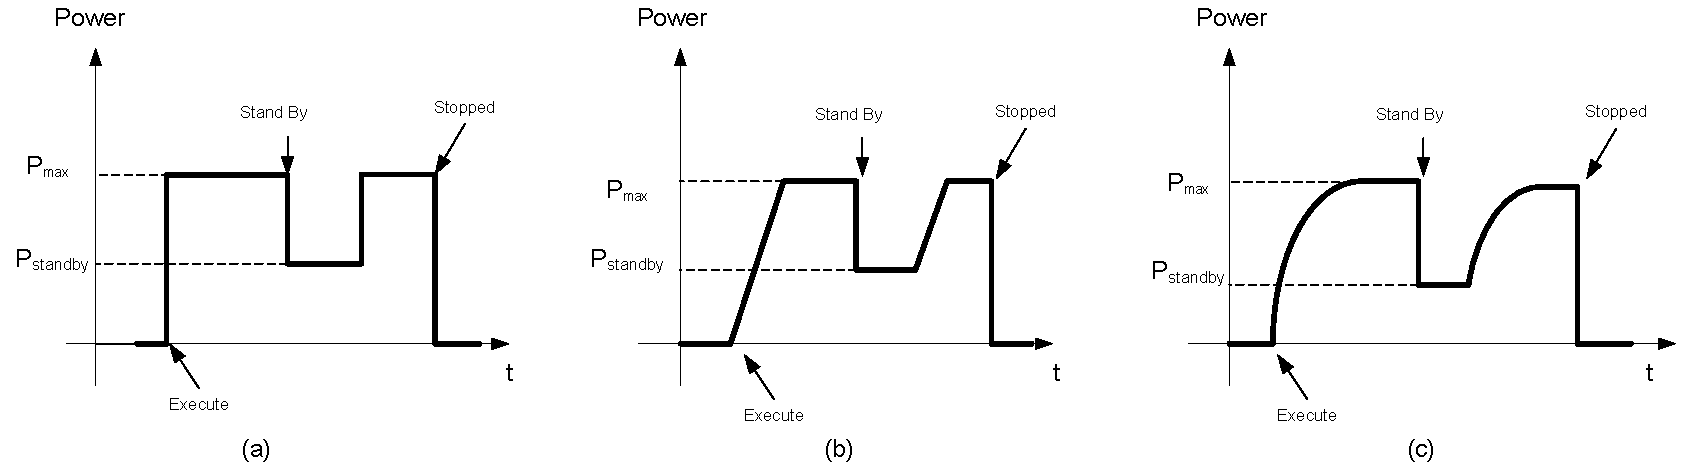
\includegraphics[scale=.40]{images/load_profile}
%
% If no graphics program available, insert a blank space i.e. use
%\picplace{5cm}{2cm} % Give the correct figure height and width in cm
%
\caption{Basic load profiles of the energy loads. In $execute$-state,  the electrical power consumed $P_i$ can be constant and equal to $P_{max}$ (a), increase linearly (b) or exponentially (c) to $P_{max}$.}
\label{fig:load_profile}       % Give a unique label
\end{figure}

 
\item{\textit{\textbf{Regenerative energy consumers}} are energy consumers with the exception that these consumers can recuperate energy for a small period of time (less than a minute). In this case we consider the load to be constant and negative. Fig. \ref{fig:recuperative_load_profile} shows a typical load profile.}

 % For figures use
%
\begin{figure}[h!]
\sidecaption
% Use the relevant command for your figure-insertion program
% to insert the figure file.
% For example, with the graphicx style use

\includegraphics[scale=.40]{images/Recuperative_Energy_Load_Profile}
%
% If no graphics program available, insert a blank space i.e. use
%\picplace{5cm}{2cm} % Give the correct figure height and width in cm
%
\caption{Basic load profiles of regenerative energy consumers. In $execute$-state,  the electrical power consumed $P_i$ can be negative for a short period of time.}
\label{fig:recuperative_load_profile}       % Give a unique label
\end{figure}


\item{\textit{\textbf{Auxiliary processes}} are energy consumer processes in the factory floor that do not execute a manufacturing task directly, but are required by the production task. These are for example compressors or cooling systems. Auxiliary processes have two required states: $off$ and $on$.}

\item{The \textit{\textbf{grid component}} represents the main grid and is responsible for buying/selling electricity from/to the main grid. It has three state: $buying$, $selling$, $idle$. If the grid agent is in $idle$-state or in $off$-state, the industrial micro-grid can be considered to be executed in isolated mode because there are no interaction with the main grid.}
\end{itemize}

\subsection{Problem Formulation}
The main objective is to minimize the total cost the energy bought from the main grid to achieve a high productivity while considering future energy prices and weather dependent renewable energy generators. Let $\mathrm{M}$ denotes the set of components of the micro-grid (or controllable machine components), such that $M_i \in \mathrm{M}, \forall i \in [0, M-1]$  with $ M \in \mathbb{N}$. We assume that each component $M_i$ can take an energy state $s_{i,t}$ (i.e. “stopped”, “running”, “aborted”, “standby”, etc.) at the time step $t  \in \mathbb{N}$ and the dynamic power consumption $P_i^t$ of $M_i$ solely depends on the current state $s_{i,t}$ of the component and the current time step $t$: $P_i^t=P_i (t, s_{i,t})$. The total energy requested/sold from/to the main grid $E_i^t$ at time interval $\triangle t$ over the complete time horizon $T \in \mathbb{N}$ is therefore the sum of the power consumed/generated of all components during the time horizon. Please notice that $P_i^t$ can also be negative in the case of renewable energy sources or regenerative energy consumers for example.

%
\begin{equation}
E_i =\sum_{t=0}^{T-1}{ P_i^t \cdot \triangle t}, \forall i \in [0, M-1]
\end{equation}
%

 If $\lambda_t^- \in \mathbb{R}$ is the actual energy price and $\lambda_t^\sim \in \mathbb{R}$ the forecasted energy price at a time step $t$, the optimization problem can be formulated for the time horizon $T$ as follow:

%
\begin{equation}
\label{eq:problem}
minimize \sum_{k=0}^{t}{ {\lambda_t^-} \cdot ({ \sum_{i=0}^{M-1}{ P_i (k, s_{i,k}) \cdot \triangle t } })}+  \sum_{l=t+1}^{T-1}{\lambda_t^\sim \cdot ({ \sum_{i=0}^{M-1}{ P_i (l, s_{i,l}) \cdot \triangle t  } }) }
\end{equation}

If $a_l (s_{i,l-1},s_{i,l})$ denotes the action of changing the state of the component $M_i$ at time $l$ from the state $s_(i,l-1)$ to the state $s_(i,l)$, the Eq. \ref{eq:problem} can be rewritten as follow:

\begin{equation}
\label{eq:problem_reformulated}
minimize \sum_{k=0}^{t}{ {\lambda_t^-} \cdot ({ \sum_{i=0}^{M-1}{ P_i (k, s_{i,k}) \cdot \triangle t } })}+  \sum_{l=t+1}^{T-1}{\lambda_t^\sim \cdot ({ \sum_{i=0}^{M-1}{ P_i (l, a_l (s_{i,l-1},s_{i,l})) \cdot \triangle t  } }) }
\end{equation}

Several constraints should be taken into consideration. One of them is the power balance between the energy demand of the micro-grid and the energy supply from the main grid:

\begin{equation}
\label{eq:constraint_energy_balance}	
	\sum_{i=0}^{M-1}{ E_i} \leq E_{max}^\sim,  \forall i \in [0, M-1]
\end{equation}
where $E_i$ denotes the total energy demand of the micro-grid component $M_i$ over the time horizon $T$ and $E_{max}^\sim$ the total available energy from the main grid.

In addition, the total energy consumption of the micro-grid at each time interval $t$ should satisfy the upper and lower bound given by the overall load profile and a tolerance interval. This constraint can be expressed as follows:

\begin{equation}
\label{eq:constraint_load_profile}	
	L_{target}^\sim - \triangle L^\sim \leq {\sum_{i=0}^{M-1}{ P_i (t, s_{i,t})} } \leq L_{target}^\sim + \triangle L^\sim
\end{equation} 
with $L_{target}^\sim$  being the target load at time step $t$, $\triangle L^\sim$  a symmetric tolerance around $L_{target}^\sim$ and $ i \in [0, M-1]$

As expressed above, solving the optimization problem is equivalent to compute at each time step the optimal state (by choosing the action $a_l (s_{i,l-1},s_{i,l})$ ) so that the resulting total energy cost of the micro-grid for a complete time horizon is globally minimized. If every component of the micro-grid is controlled by an agent, then the optimization problem is equivalent to finding a coordinated strategy for all the agents. In this case, the main challenge lies in the volatility of future energy prices and the direct dependence of future energy consumption from actual decisions. Furthermore, other constraints such as the the throughput, production time, the product quality, the production cost, etc. have to be considered.

\subsection{Markov Game Formulation}
The formulated optimization problem can be transformed into a reinforcement learning task, where each agent controlling a component of the grid has to learn a policy that maximizes a cumulative reward signal derived from the objective function and is conditioned by the constraints formulated in Eq. \ref{eq:constraint_energy_balance} and Eq. \ref{eq:constraint_load_profile}. 

If we consider the global state of the environment as the aggregation of the observations of all agents, then the observed state of the environment solely depends on the actions of all the agents and the previously observed global state of the environment. In other words, no external factors besides the actions of all the agents will affect the dynamics of the environment. Under this assumption, the multi-agent reinforcement-learning task satisfies the Markov property and can be therefore formulated as a Markov decision process (MDP).

In this work, we consider a multi-agent extension of Markov decision processes called observable Markov games \cite{Littman1994multiagent}. A Markov game for $N$ agents is defined by a set of states $\mathrm{S}$ describing the possible configurations of all agents, a set of actions $\mathrm{A}_1, \mathrm{A}_2, \ldots, \mathrm{A}_N$ and a set of observations $\mathrm{O}_1,\mathrm{O}_2, \ldots, \mathrm{O}_N$ for each agent. To choose actions, each agent $i ( i= 1,2,\ldots, N)$ uses a stochastic policy $\pi_{\theta_i} : \mathrm{O}_i \times \mathrm{A}_i \mapsto [0; 1]$, where $\theta_i$ are the parameters of the policy. The policy produces the next state according to the state transition function $T : \mathrm{S} \times  \mathrm{A}_1 \times ...  \times \mathrm{A}_N \mapsto \mathrm{S}$. Each agent $i$ obtains rewards as a function of the state and agent’s action $r_i : \mathrm{S} \times \mathrm{A}_i  \mapsto \mathbb{R}$, and receives a private observation correlated with the environment state $o_i : \mathrm{S} \mapsto \mathrm{O}_i$. The initial states are determined by a distribution  : $\mathrm{S} \mapsto [0; 1]$. Each agent $i$ aims to maximize its own total expected return $R_i = \sum_{t=0}^{T}{\gamma^t \cdot r_i^t}$ where $\gamma^t$ is a discount factor at time step $t$ and $T$ is the time horizon. The \textit{action-value function} is defined as $\mathrm{Q}^{\pi_i}(s_{i,t}, a_t^i)=\mathbb{E}[\mathrm{R}_i^t|s_{i,t},a_t^i]$, while the \textit{state-value function} is defined as $\mathrm{V}^{\pi_i}(s_{i,t})=\mathbb{E}[\mathrm{R}_i|s_{i,t}]$. The
\textit{advantage function} $\mathrm{A}^{\pi_i}(s_{i,t}, a_t^i) = \mathrm{Q}^{\pi_i}(s_{i,t}, a_t^i) - \mathrm{V}^{\pi_i}(s_{i,t})$ describes whether taking action $a_t^i$ is better or worse for agent $i$ when in state $s_{i,t}$ than the average action of policy $\pi_{\theta_i}$.

For our micro-grid, we provide a uniform representation of the operational state of the grid components which is illustrated in Fig. \ref{fig:state_chart}. The state space of every agent is represented by the operation state of the grid component it controls aggregated with the target load of the grid, the current  time step within  the production shift, the amount of production tasks to execute as well as the current energy price. Notice that we do not assume inter-dependencies between the production tasks. The action space of each agent is represented by all the actions that can change the operational state of a grid component (See Fig. \ref{fig:state_chart}). The reward of each agent depends on the type of the grid component it controls and therefore is use case dependent. See Eq. \ref{eq:total_reward} in section \ref{subsec:42} for more details.

 % For figures use
%
\begin{figure}[h!]
%\sidecaption
% Use the relevant command for your figure-insertion program
% to insert the figure file.
% For example, with the graphicx style use
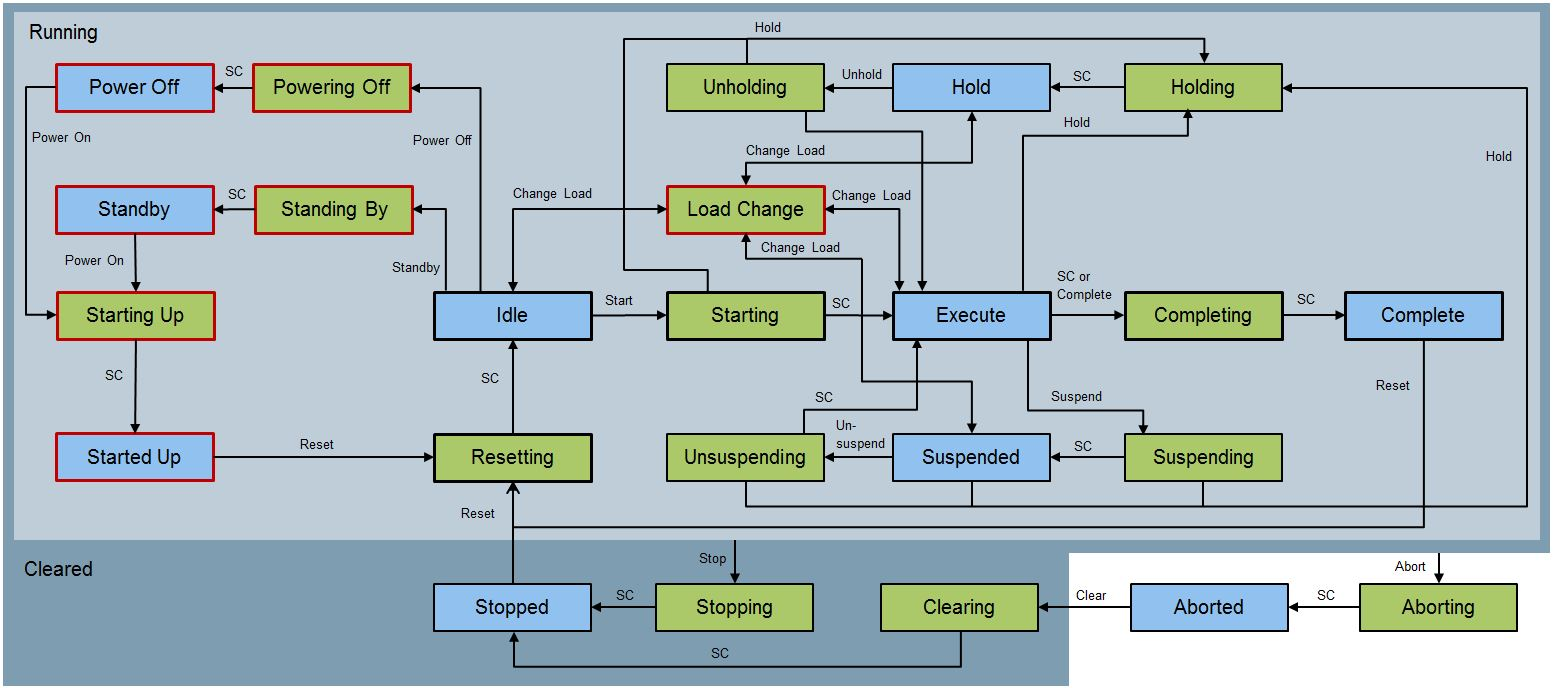
\includegraphics[scale=.40]{images/StateMachine_EFlex}
%
% If no graphics program available, insert a blank space i.e. use
%\picplace{5cm}{2cm} % Give the correct figure height and width in cm
%
\caption{Uniform state representation of a grid component. Every component can be stopped, halted, suspended, powered up or aborted. Once the component reach the $execute$-state then it begins to execute a production task, to generate energy or to store/release energy.}
\label{fig:state_chart}       % Give a unique label
\end{figure}





\section{Approach}
\label{sec:4}
\subsection{Multi-Agent Proximal Policy Optimization}
\label{subsec:41}

Since the naive application of standard reinforcement learning algorithms performs poorly in multi-agent settings, our goal is to derive an algorithm that can operate under the following constraints:
\begin{itemize}
\item{The learned policies can only use local information (i.e. own observations) at execution time.}
\item{There is no particular communication method between the agents, since it can restrict the scalability of the solution.}
\item{We do not assume a differential model of the environment dynamics.}
\end{itemize}
Fulfilling the above desiderata would provide a general-purpose multi-agent learning algorithm that could be applied not just to cooperative games with explicit communication channels, but also to competitive games and games involving only physical interactions between agents.

We accomplish our goal by adopting the framework of centralized training with decentralized execution in which agent policies are composed of two separate networks with different parameters: a policy network (actor) that generates an action distribution and a critic network (critic) that predicts discounted future returns. The critic uses extra information to ease training process whilst actors take actions based solely on their own local observations. This is still a valid approach as long as the information used during the training of the agents are not used at test/execution time.

% For figures use
%
\begin{figure}[h!]
%\sidecaption
% Use the relevant command for your figure-insertion program
% to insert the figure file.
% For example, with the graphicx style use
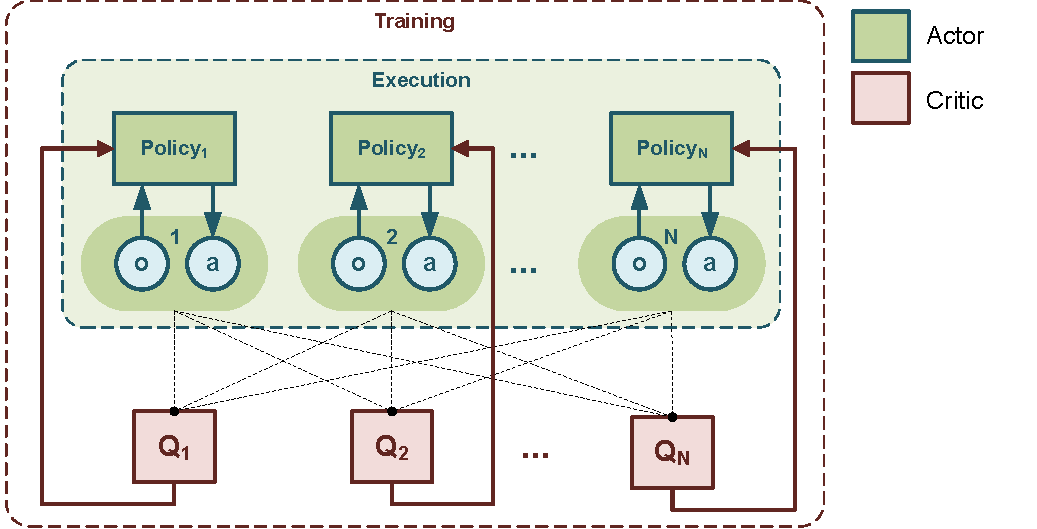
\includegraphics[scale=.65]{images/MAPPO}
%
% If no graphics program available, insert a blank space i.e. use
%\picplace{5cm}{2cm} % Give the correct figure height and width in cm
%
\caption{Overview of our multi-agent decentralized actor, centralized critic approach. The centralized action-value function (critic) for each agent takes as input the actions and observations of all agents and predicts the discounted future returns (Q-values) for the agent while the actor produces an action distribution based solely on the agent's observations and actions.}
\label{fig:MAPPO}       % Give a unique label
\end{figure}

As illustrated in Fig. \ref{fig:MAPPO}, our centralized action-value function (critic) for each agent takes as input the actions and observations of all agents and predicts the discounted future returns for the agent. Additional information can also be included in the inputs. Since each action-value function is learned separately, each agent can have arbitrary rewards including conflicting rewards in competitive scenarios.

Furthermore, we extend the idea of \cite{schulman2017proximal} by adopting the proximal policy optimization algorithm (PPO) as the main policy optimization algorithm instead of deep deterministic policy gradient (DDPG) as presented in the paper. PPO is a family of policy optimization methods that use multiple epochs of stochastic gradient ascent to perform each policy update. It performs comparably to or better than DDPG while being much simpler to implement and tune.

\subsection{Cooperation and Competition}
\label{subsec:42}
As we seek the emergence of coordination strategies between the components of the micro-grid, the agents controlling the mico-grid components are trained using \textit{self-play} in an \textit{autocuricula} configuration. This acts as a natural curriculum as these agents are always in a mixed cooperative and competitive setting. For example, the energy loads (i.e. production machines) of the micro-grid are always in competitive settings. If there is not enough electrical energy available in the grids, then some production machines have to turn themselves off so that the production can be carried on by the other machines. In the same direction, cooperation can take place if, for example, the energy storage components need to be switched on in order to increase the electrical energy available in the energy bus and thus enable the production machines to perform additional production tasks.

Adopting such a configuration also offers many advantages. If a new successful strategy is adopted by an agent, it implicitly changes the task distribution for the competing agents which are then forced to develop a better strategy. These evolutionary arms races create an implicit autocurriculum in which competing agents constantly create new tasks for each other and thus discover new powerful and robust strategies and counter-strategies. In addition, the multi-agent autocurriculum is open-ended. That means that the training will only stabilizes once equilibrium between the different agents is founded which can only be reached if a suitable coordination strategy between the agents has emerged. Due to the exploration factors, many coordination strategies can also emerged at different stages of the training.

In order to create a competitive setting, competing agents are rewarded with competitive rewards. If an agent wins the game, it receives a positive reward and all other competing agents are penalized by an opposite negative reward. If nobody wins the game, then all competing agent are penalized. In a cooperative setting, agents are given a team based reward; meaning that all members of the team receive a positive rewards, if a team member wins the game. To confine agent behavior to a reasonable space, we also introduced an environmental-based penalization.

The success of agents in the autocuricula setting requires the agents to occasionally solve the task (win the game) by random actions. The probability of this happening in most games is minuscule as they require as a prerequisite some fundamental skills like the ability to properly control the operational state machine of the grid component. For example the agent must first quickly learn how to bring a production machine in the $execute$-state in order to start a production task or how to turn on/off the storage component without suspending/halting the production. To overcome this problem, we use simple dense rewards at each step so that the agents can first learn basic motor skills that increase the likelihood that random actions of the agent will result in a relatively small positive reward. We refer to this reward as the \textit{exploration reward}. The exploration reward is then gradually annealed to zero, in favor of the \textit{competition/cooperation reward}, to allow the agents to learn coordination strategies for the remaining training time. This is achieved using a linear annealing factor $\alpha$. We also introduce an \textit{environmental reward} which aims to penalize action sequences leading to dangerous outcomes (for example system configurations violating the constraints formulated in Eq. \ref{eq:constraint_energy_balance} and Eq. \ref{eq:constraint_load_profile}) and a \textit{productivity reward} which encourage production machines to execute production tasks more frequently. 

So, at time-step $t$, if the exploration reward is $r_{explo}$, the competition reward is $r_{comp}$, the environmental reward $r_{env}$, the the productivity reward $r_{prod}$ and T is the termination time-step, then the total agent reward is:
\begin{equation}
\label{eq:total_reward}	
	r_t = \alpha \cdot r_{explo} + (1 - \alpha) \cdot (r_{comp} + r_{env} + r_{prod})
\end{equation} 

With this formulation, the agents are trained initially on the dense reward for only about 10-20\% of the training epochs in order to gain some basic skills first. 


\section{Experiments}
\label{sec:5}
Our aim is to show that the agents controlling an industrial micro-grid can learn complex behaviors and coordination strategies that can lead to an optimization of the global energy consumption. Therefore, we train the agents in different competitive and cooperative scenarios. In each scenario, the environment consists of multiples agents with discrete action space, discrete time space and mixed observation spaces. Every agent controls a grid component and may take physical actions in the environment by changing the operational state of the corresponding grid component. We do not assume that all agents have identical action and observation spaces, or act according to the same policy $\pi_{\theta}$. The environment of each experiment were implemented as an extension of OpenAI environment Gym \cite{Brockman01540}. We found this framework useful for creating environments involving complex interaction between agents, while keeping the control and perception problems simple, as we are primarily interested in addressing agent strategies. 

Unless otherwise specified, the actor and the critic of each agent is parameterized by a two-layer ReLU MLP with respectively $256$ units per layer for the actor and $512$ units per layer for the critic. In all of our experiments, we use the Adam optimizer with a learning rate of $0.0001$ and the discount factor $\gamma$ is set to be $0.9$. The size of the replay buffer is $10240$ and the sampling time horizon is $1024$. We update the network parameters after every $1024$ sampling steps and we use a batch size of $512$. We train with $10$ random seeds for environments with stark success/fail conditions (\textit{experiment 2} and \textit{experiment 3}) and with only $2$ seed for \textit{experiment 1}. For the PPO-algorithm, we set the clipping parameter $\epsilon$ to $0.1$, the entropy coefficient to $0.005$ and the exploration noise to $0.2$.

This section describes in details the designed experiments as well as the specific training parameters and analyzes various aspects of the learned behaviors. Codes for the environments as well as learned policy parameters of the agents in all environments are open-sourced and available at \cite{Bakakeu2019}.

\subsection{Experiment 1: Autocurricula and Emergent Behavior}
\label{subsec:51}
In this scenario, we consider a micro-grid of $4$ identical production machines (energy loads) executing the same production task. The grid is operated in connected mode. However, the main grid can only provide enough energy for $3$ production machines to operate. Therefore, the production machines are in full competition. The exploration reward of the agents is set so that the agent is penalized if the production machine is shouted down or suspended. The competition reward is based on the performance of the machines meaning that the agent will receive a positive incentive every time a production task is accomplished. In addition, all agents are penalized if the total energy demand is greater than the energy provided by the main grid. The exploration annealing factor $\alpha$ is set to $0.2$ so that the agent will first learn how to execute a production task during the initial $20\%$ of the training time. During the training each agent observed the full environment including the observations and the actions of the other agents. During the execution, the agents only observe the amount of energy available as well as the current operational state of the machine it controls. We train the agents with $2$ random seeds for $500$ sampling horizons.

% For figures use
%
\begin{figure}[b]
\sidecaption
% Use the relevant command for your figure-insertion program
% to insert the figure file.
% For example, with the graphicx style use
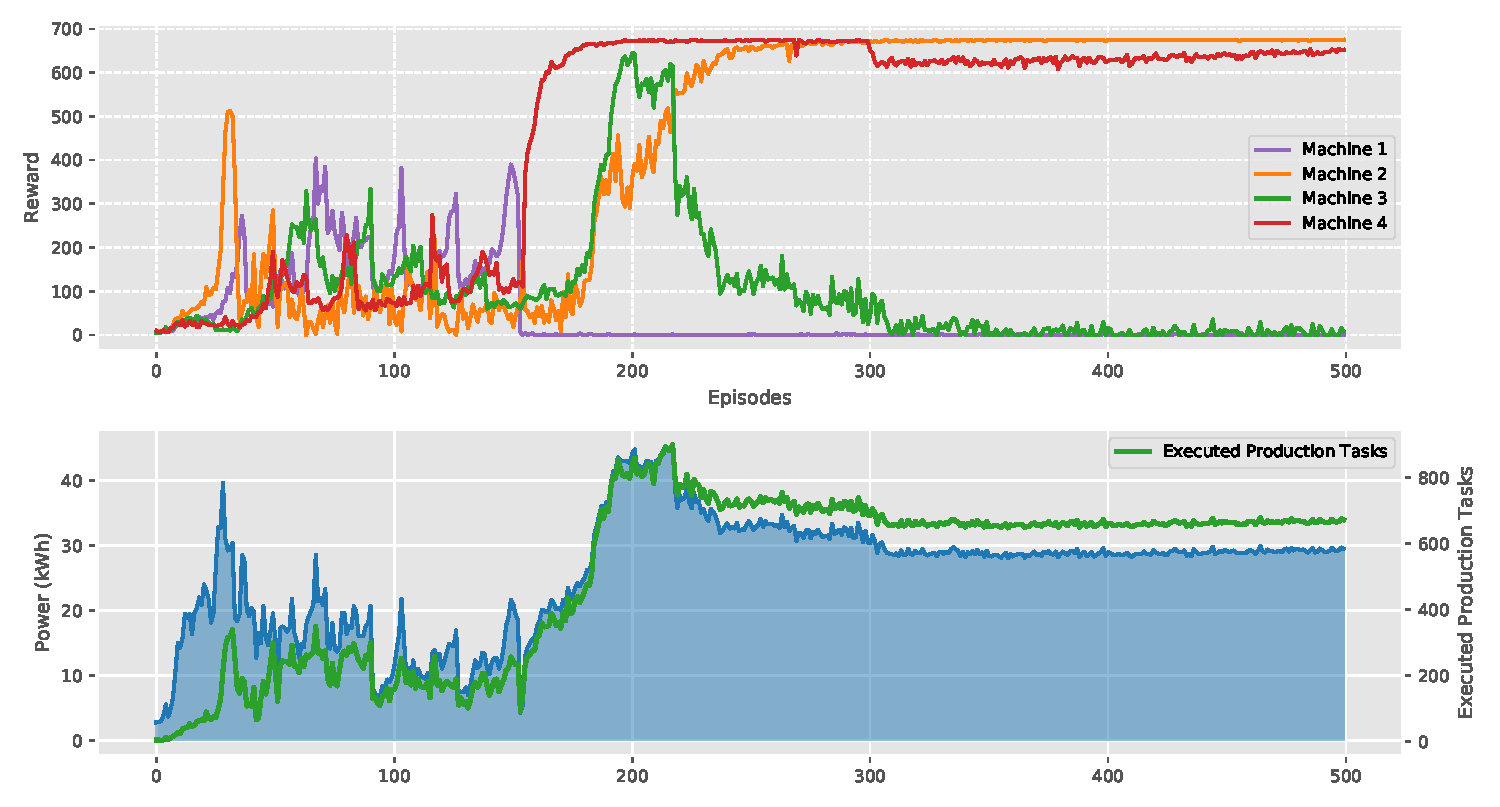
\includegraphics[scale=.48]{images/experiment_1_results}
%
% If no graphics program available, insert a blank space i.e. use
%\picplace{5cm}{2cm} % Give the correct figure height and width in cm
%
\caption{Emergent Skill Progression From Multi-Agent Autocurricula. Through the reward signal
agents go through different distinct stages of emergence. (a) Episode 1-30: the different agents learn basic skills (how to execute a production task) and the productivity rise. (b) Episode 30-160: strategy exploitation and competition take place between the agents and stabilize only when \textit{machine 1} adopts a very bad strategy. (c) Episode 160-220: the first coordination strategy emerge. \textit{Machine 2}, \textit{Machine 3} and \textit{Machine 4} start to produce more frequently while \textit{Machine 1} remains in the $idle$-state more often. (d) Episode 220-500: a second coordination strategy emerge.  \textit{Machine 2}, \textit{Machine 4} reached their highest productivity while \textit{Machine 3} is frequently halted.}
\label{fig:scenario_1_results}       % Give a unique label
\end{figure}

Fig. \ref{fig:scenario_1_results} shows a typical progression of the emergent strategies learned by all agents during the course of the training measured in this case by the respective average cumulative rewards. Clearly, training the agents against each other creates many different strategies, each of which introduces a previously non-existent pressure on other agents to do better in order to move to the next stage. Note that there are no direct incentives for agents to explore, but rather the emergent strategies are solely a result of the auto-curriculum induced by multi-agent competition.

Fig. \ref{fig:scenario_1_results} shows a typical progression of the emergent strategies. Initially, the agents learn simultaneously how to control the corresponding production machine so that it can reach the $execute$-state as often as possible. After approximately 30 episodes, all agent have mastered this task and the energy demand of the whole grid begin to surpass the energy provided by the main grid. Consequently, the agents are then frequently penalized leading to a significant reduction of the production performance and the accumulated reward. At this point some agents begin to take advantage of the observations and actions of other agents and intentionally modify their policies accordingly. We can see , for example, some agents wait in the $idle$-state and then switch to the $execute$-state, when other agents are stopped or halted. However, the more the new strategy becomes efficient, the more it becomes predictable and the other agents begin to defend themselves against this strategy. After another 5-20 episodes, all agents have now learned to exploit the strategy of other agents and the energy demand of the production machines again surpass the energy supply and the agents are penalized again more frequently. At this point a new adaptation/exploitation cycle restarts. Because of random exploration factors, the best performing agent during this phase changes from cycle to cycle. After approximately 3-6 cycles (which corresponds to episode 30 - 160), the training stabilized when at least one agent adopts a very bad policy e.g. only switching between $stopped$- and $idle$- state. The first acceptable coordination strategy emerges from episode 160 to approximately episode 220: \textit{Machine 2}, \textit{Machine 3} and \textit{Machine 4} start to produce more frequently while \textit{Machine 1} remains in the $idle$-state oftenly. It is a valid strategy since the energy required for the production can be supplied by the main grid and the overall productivity is  relatively high. The second and final coordination strategy emerge at episode 220: while \textit{Machine 2} and \textit{Machine 4} reached their highest productivity,  \textit{Machine 3} is frequently halted.

In this experiment, we found that the emergent auto-curriculum is fairly robust, as similar observations can be made with different initialization strategies. Out of $10$ experimental runs, more than $7$ runs were able to converge to an equilibrium. However, many design choices can drastically reduce the convergence time and the sample complexity such as the surrogate loss and the entropy loss of the underlying PPO-algorithm. We also experimented with different configurations (for example by including energy storage and generator components) and found that these configurations also lead to emergent behaviors, providing further evidence that multi-agent interaction is a promising path towards self-supervised energy management.

\subsection{Experiment 2: Fully Cooperative Production}
\label{subsec:52}

% For figures use
%
\begin{figure}[h!]
\sidecaption
% Use the relevant command for your figure-insertion program
% to insert the figure file.
% For example, with the graphicx style use
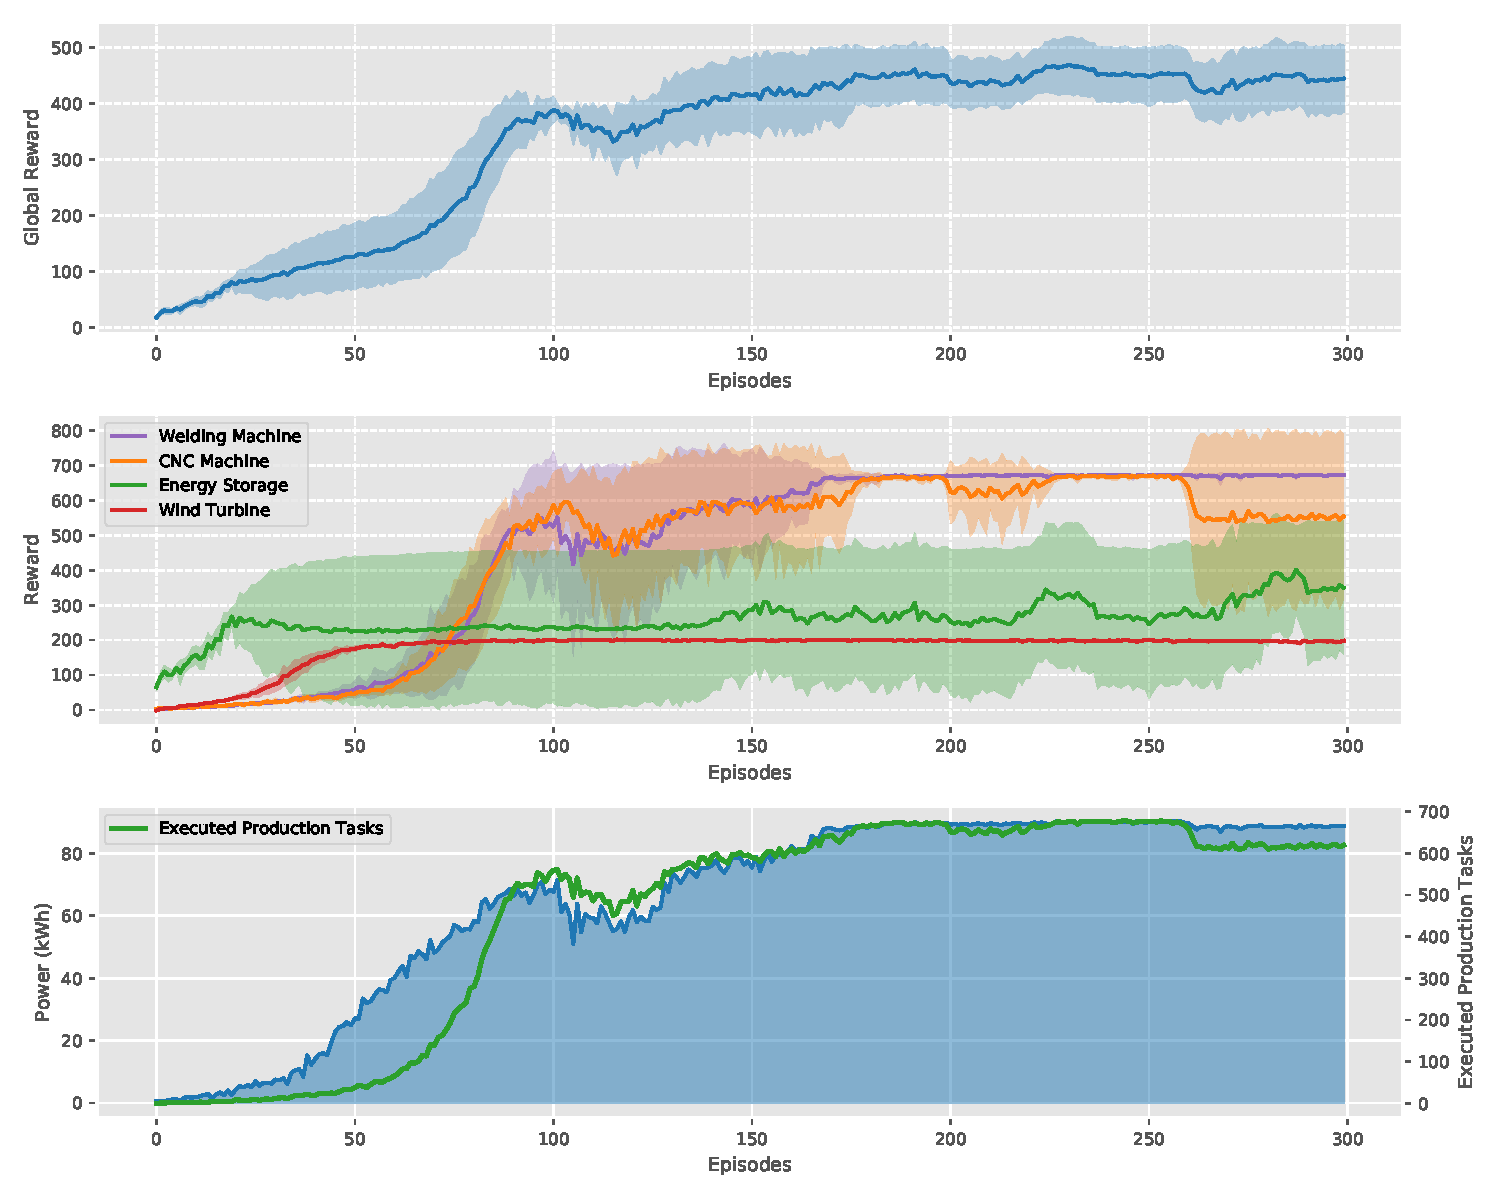
\includegraphics[scale=.48]{images/experiment_2_results}
%
% If no graphics program available, insert a blank space i.e. use
%\picplace{5cm}{2cm} % Give the correct figure height and width in cm
%
\caption{Average rewards on cooperative production. A coordination strategy emerges rapidly after $100$ episodes. While the energy generators rapidly learn how to generate energy, the energy storage component adopted to discharge when the production machines in the $execute$-state and thus allowing the production machine to increase the productivity.}
\label{fig:scenario_2_results}       % Give a unique label
\end{figure}

In this scenario, the micro-grid is operated in isolated mode and consists of two production machines (a CNC-machine and a welding machine), an energy generator (a wind turbine) and an energy storage system. The energy generated by the wind turbine is lower than the energy needed by the production machines. Therefore, the energy storage system has to be turned on in order to execute a production task. All the components should therefore cooperate. The exploration rewards is similar to the previous experiment and the team-based cooperation reward of the agents is based on the performance of the production machines. We train the agents for $300$ episodes. The agents also used the same policy network architecture as in experiment 1 (see section \ref{subsec:51}).

As we can observe in Fig. \ref{fig:scenario_2_results}, the components rapidly learn the required basic skills and a coordination strategy emerge around the episode $100$. While the energy generator is constantly switched on, the energy storage component learns to charge when the production machines are standing still and to discharge when the production machines perform a production task and thus supports production. Once the energy generator and the energy storage component have adopted a strategy, the production machines rapidly learn to increase their productivity which reach its highest level around episode $250$.

To determine the seed dependence of the skill emergence, we ran this environment with $10$ random seeds and looked at the variability of the onset of behavioral shifts across runs. We find that the behavioral shifts happen at very similar times around episode $100$ in training. Rewards and environment statistics are very consistent in early as well as in later times in training.

\subsection{Experiment 3: Effect of Exploration Curriculum}
\label{subsec:53}
... yet to come!!! [TODO: Jupiter Bakakeu]


\section{Conclusion and Future Work}
\label{sec:6}
This chapter presents an artificial intelligence algorithm especially a multi-agent reinforcement algorithm for the energy optimization of an heterogeneous cluster of flexible manufacturing machines with energy generation and energy storage capabilities in an electricity micro grid featuring a high volatility of electricity prices. It demonstrated that simple game rules, multi-agent competition, and standard reinforcement learning algorithms at scale can induce agents to learn complex coordination strategies and skills that can lead to an optimization of the global energy consumption while ensuring a high productivity. 

We analyze the performance of the proposed approach with respect to the number of agents and the micro-grid configuration in mixed cooperative and competitive scenarios and found that different production machines were able to discover different coordination strategies in other to increase the energy efficiency of the whole factory floor. These empirical results are promising and we intend to extend the solution to highly complicated and dynamic environments.

The presented results should be viewed as a proof of concept showing that multi-agent autocurricula can lead to physically grounded coordination strategies. We acknowledge that the strategy space in the proposed environments are inherently bounded and do not reflect the reality of the factory floor since many factors such as product quality, the production time and the unexpected human interventions in the production process have to be considered. However, because the algorithm was built on the functional abstraction of cyber-physical production systems, it is therefore applicable to real production systems if an invocation interface is connected to the agents. Our solution is therefore physically grounded and very extensible. In order to support further research, we have open-sourced our environment code \cite{Bakakeu2019}.


\begin{acknowledgement}
The authors would like to thank Joern Pechke, Hans-Henning Klos, Shirin Baer, and others at Siemens AG for interesting discussions related to this paper, as well as Matthias Brossog, Jonathan Fuchs and Dominik Kisskalt for the insightful comments on this manuscript. Finally, we’d like to thank Siemens AG for fostering an engaging and productive research environment.

\end{acknowledgement}

%%%%%%%%%%%%%%%%%%%%%%%% referenc.tex %%%%%%%%%%%%%%%%%%%%%%%%%%%%%%
% sample references
% %
% Use this file as a template for your own input.
%
%%%%%%%%%%%%%%%%%%%%%%%% Springer-Verlag %%%%%%%%%%%%%%%%%%%%%%%%%%
%
% BibTeX users please use
% \bibliographystyle{}
% \bibliography{}
%

\bibliographystyle{ieeetr}
\bibliography{bibliography}


\end{document}
